\section{React}

Utolsóként röviden a React\footnote{\url{https://hu.reactjs.org/}} kódbázisára fogunk kitérni. A React a vue-hoz hasonlóan egy webes, JavaScript-alapú frontend könyvtár. A React erősen épít a funkcionális programozásból ismert koncepciókra és a webes világ HTML-CSS-JS szegregációjától eltér a JSX formátumával, ami ezt a hármat ötvözi.

\lstset{language=JavaScript, caption={Egy egyszerű React komponens}}
\begin{lstlisting}
import React, { useState } from 'react';

function Example() {
    return (
        <div>
            <p>You clicked {count} times</p>
            <button onClick={() => setCount(count + 1)}>
                Click me
            </button>
        </div>
    );
}
\end{lstlisting}

Az analízis rövidségének két oka van:
\begin{enumerate}
    \item A react kódbázisa több nagy refactor-on esett át, ami jelentősen megnehezíti a különböző verziók közötti kapcsolatok kialakítását. A snapshot-okat általában a különböző fájlok elérési útvonalain lehet csak összekapcsolni, mert a fájlok nevei nem egyediek, viszont az elérési útvonalak változása miatt csak egy nagyon kis szeletét lehetne megvizsgálni a projektnek
    \item A régebbi react kiadásokra nem lehet coverage report-okat generálni, mert a projekt egyik histórikus függősége egy az egyben el lett távolítva az NPM-ről biztonsági okokból
\end{enumerate}

Ennek ellenére a React kódbázisa különösen érdekes lesz, mert egy olyan jelenséget produkál, amit a Vue és a Moment.js nem.
Elsőként nézzük a React 14-es és 15-ös verziójának a legtöbbet módosított fájljait a \ref{fig:react-14-15-changes} ábrán. Eddig egyelőre nem látszik semmi különös, nagyrészt hasonló értékeket és mintákat látunk, mint a Vue és a Moment esetében.

\begin{figure}[H]
    \centering
    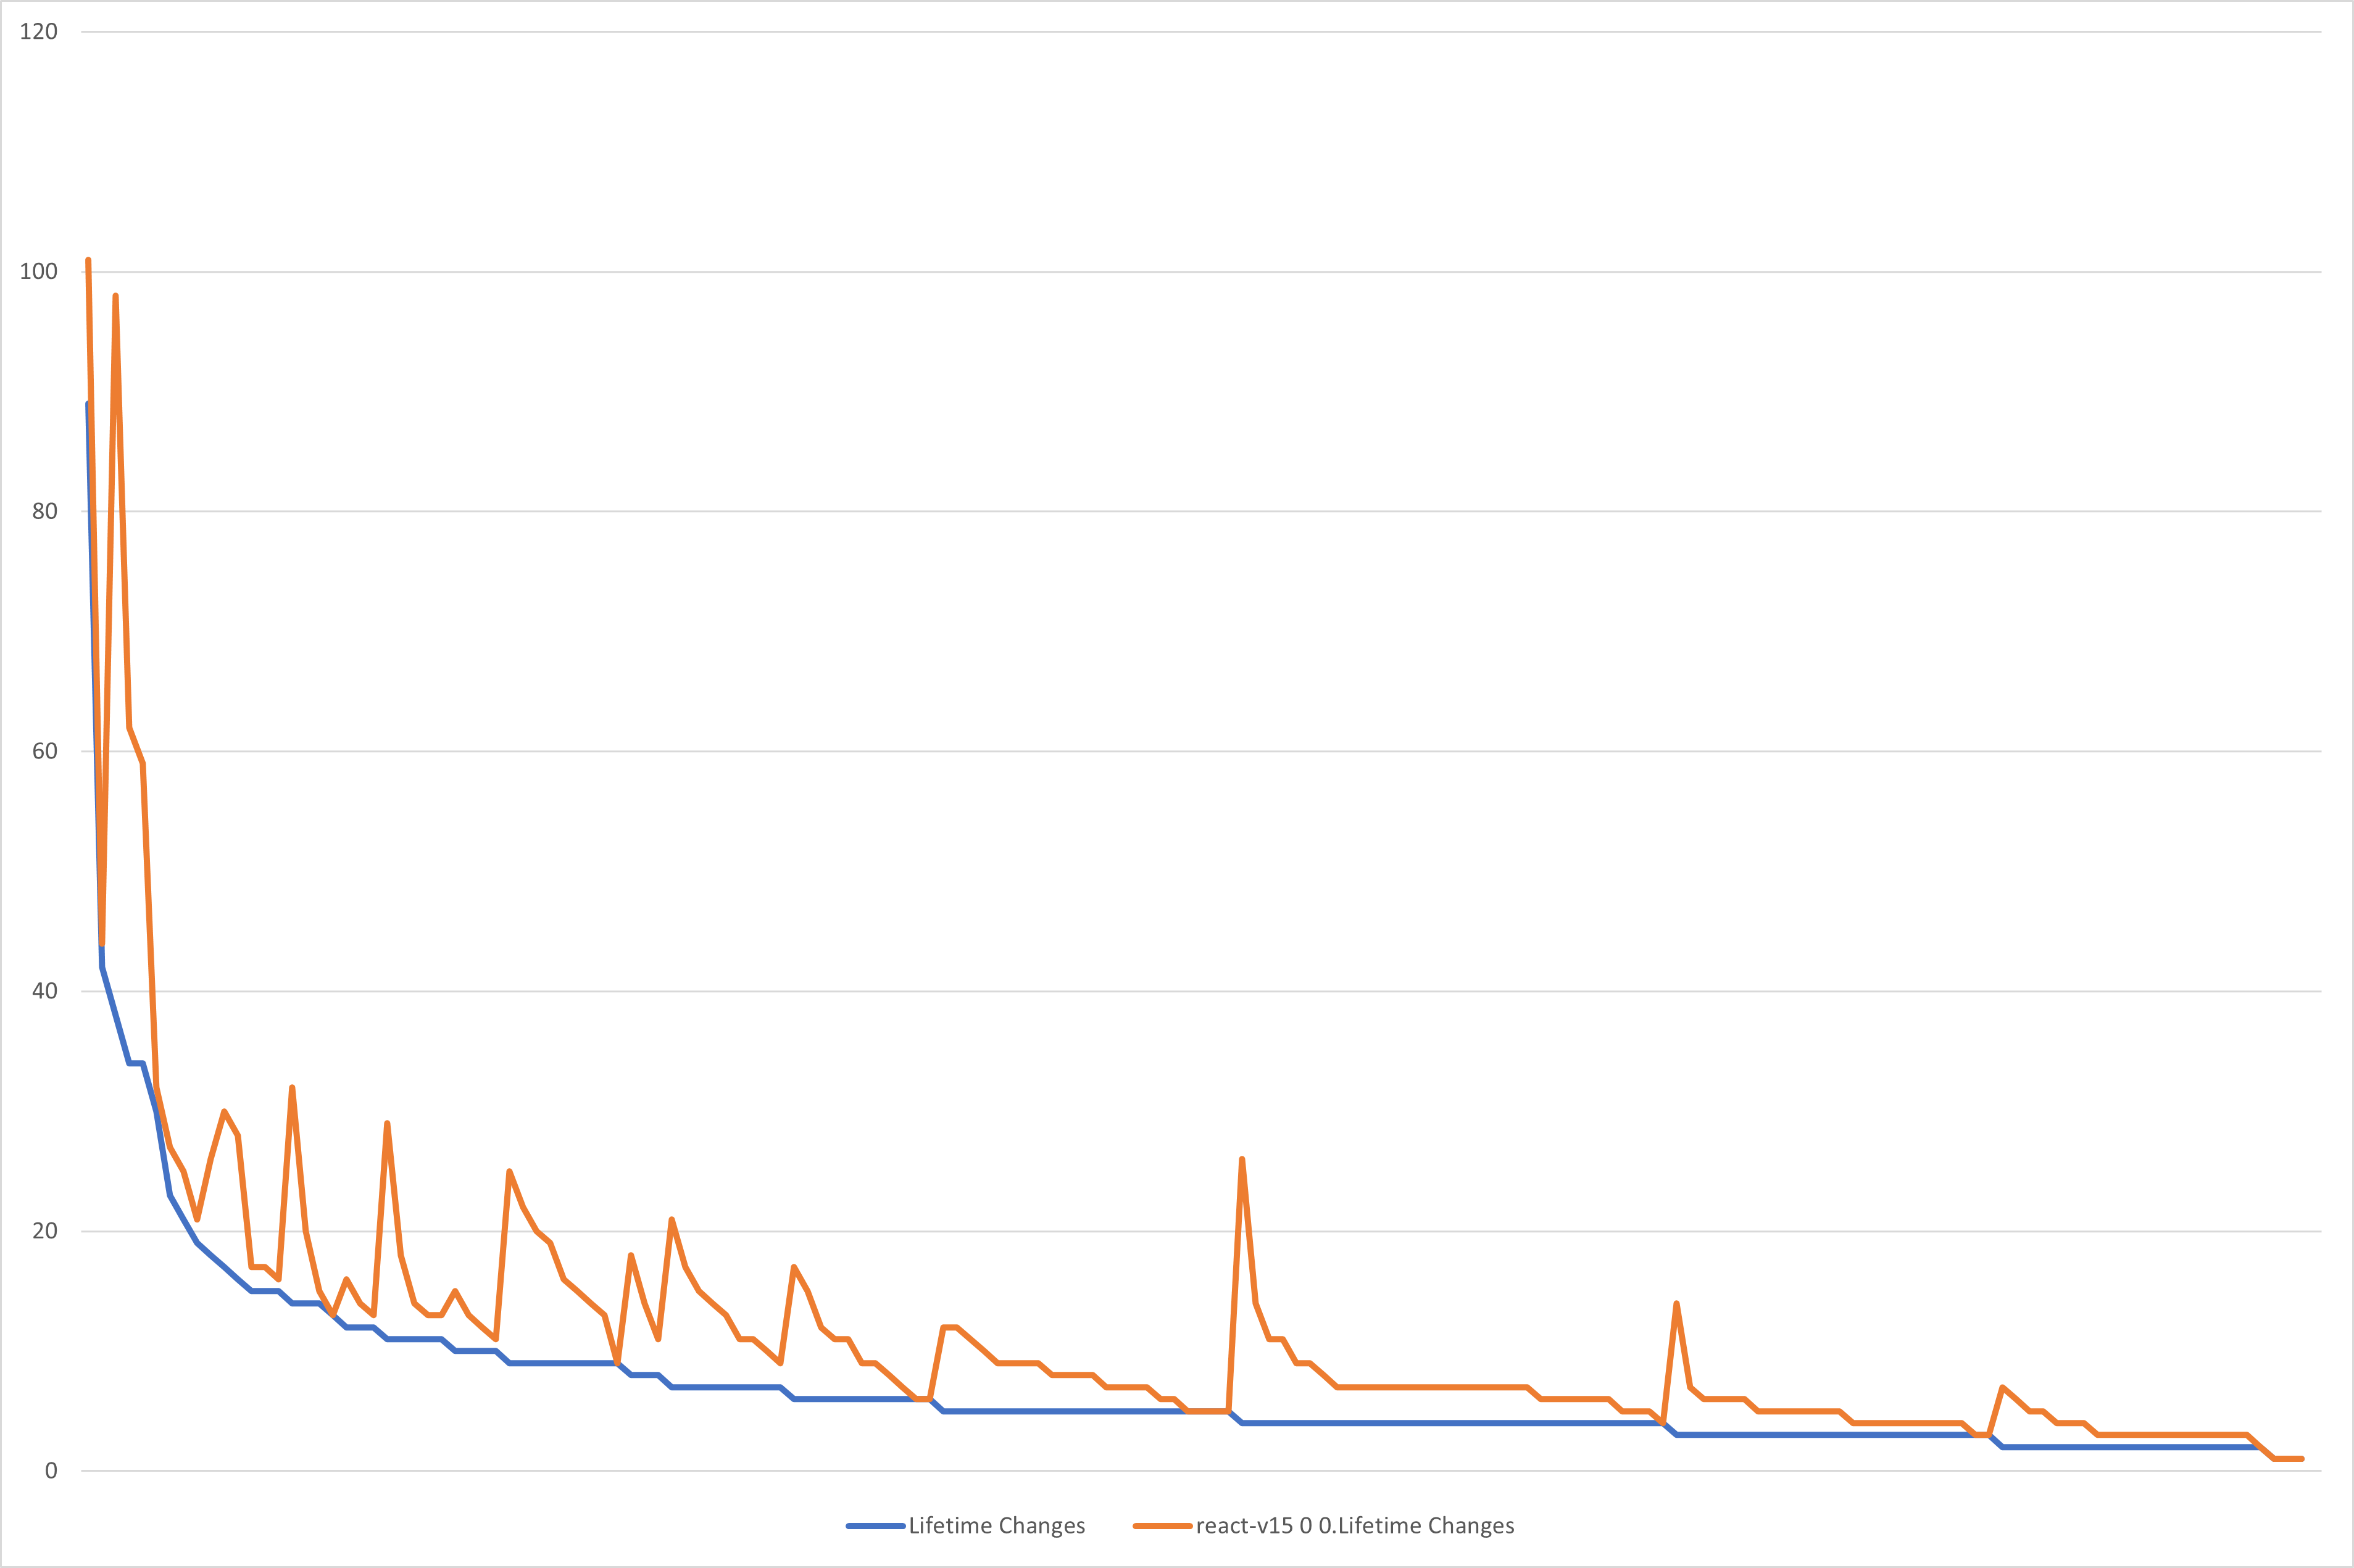
\includegraphics[width=1\textwidth]{images/react/react-14-15-changes.png}
    \caption{A React 14-es és 15-ös verziójának módosítási számai}
    \label{fig:react-14-15-changes}
\end{figure}

Vessünk azonban egy pillantást a \ref{tab:react-all-changes} táblázatra, amiben 16-os verzióban legtöbbet változtatott fájlok szerepelnek a histórikus módosítási adatokkal. Mint látható, a top 10-ben 9 olyan fájl van, amik nem léteztek a 16-os verziót megelőzően. Ez egy kis magyarázatra szorul.

A React a 16-os kiadásban egy teljes új renderelő architektúrára váltott, ami Fiber\footnote{\url{https://reactjs.org/blog/2017/09/26/react-v16.0.html\#new-core-architecture}} kódnéven futott. Nyilvánvalóan egy frontend framework legkritikusabb része a DOM rendering, amit gyakorlatilag alapjaitól írtak újra a React fejlesztői. Ugyan ez a változtatás a 16-os verzióban került be az éles kódbázisba, egy párhuzamos branch-en akkor már régóta aktív fejlesztés alatt állt.

Az eddigi megfigyelések azt mutatták, hogy amikor egy kódbázis elindul egy bizonyos irányba, akkor a korai módosítási minták medrében folyik a fejlesztés a projekt élete során. A react azonban jó példa arra, hogy ez nem feltétlenül igaz: ha a projekt új architektúrára vált, akkor ki lehet kerülni az előre lefektetett mintákat.

Ebben az esetben azonban azonban ez az új architektúra hiába cseréli le a régi, sokat módosított fájlokat, ahogy az \ref{fig:react-all-changes} ábrán látszik a Fiber architektúra pontosan ugyanazt a mintát mutatja, hiába teljesen új kód. Ez természetesen ahogy korábban a code smell-eknél tisztáztuk nem feltétlenül gond, hiszen a projekt korai hibáit javító, új központi architektúra objektíven tud emelni a projekt színvonalán.

\begin{table}[h]
    \centering
    \begin{tabular}{l|l|l|l}
        Filename                    & v14 & v15 & v16 \\ \hline
        ReactFiberScheduler.js      & 0   & 0   & 187 \\
        ReactFiberBeginWork.js      & 0   & 0   & 161 \\
        ReactFiberReconciler.js     & 0   & 0   & 114 \\
        ReactChildFiber.js          & 0   & 0   & 102 \\
        ReactFiberCompleteWork.js   & 0   & 0   & 95  \\
        ReactFiber.js               & 0   & 0   & 87  \\
        ReactFiberCommitWork.js     & 0   & 0   & 78  \\
        ReactDOMFiberComponent.js   & 0   & 0   & 77  \\
        ReactFiberClassComponent.js & 0   & 0   & 73  \\
        ReactCompositeComponent.js  & 34  & 62  & 63  \\
        ReactElement.js             & 17  & 30  & 55  \\
        ReactFiberUpdateQueue.js    & 0   & 0   & 52  \\
        DOMPropertyOperations.js    & 11  & 29  & 49  \\
        ReactElementValidator.js    & 15  & 17  & 49  \\
        HTMLDOMPropertyConfig.js    & 14  & 32  & 48  \\
        ReactFiberContext.js        & 0   & 0   & 44  \\
        ReactDOMComponent.js        & 38  & 38  & 38
    \end{tabular}
    \caption{A React 16-os kiadása}
    \label{tab:react-all-changes}
\end{table}

\begin{figure}[H]
    \centering
    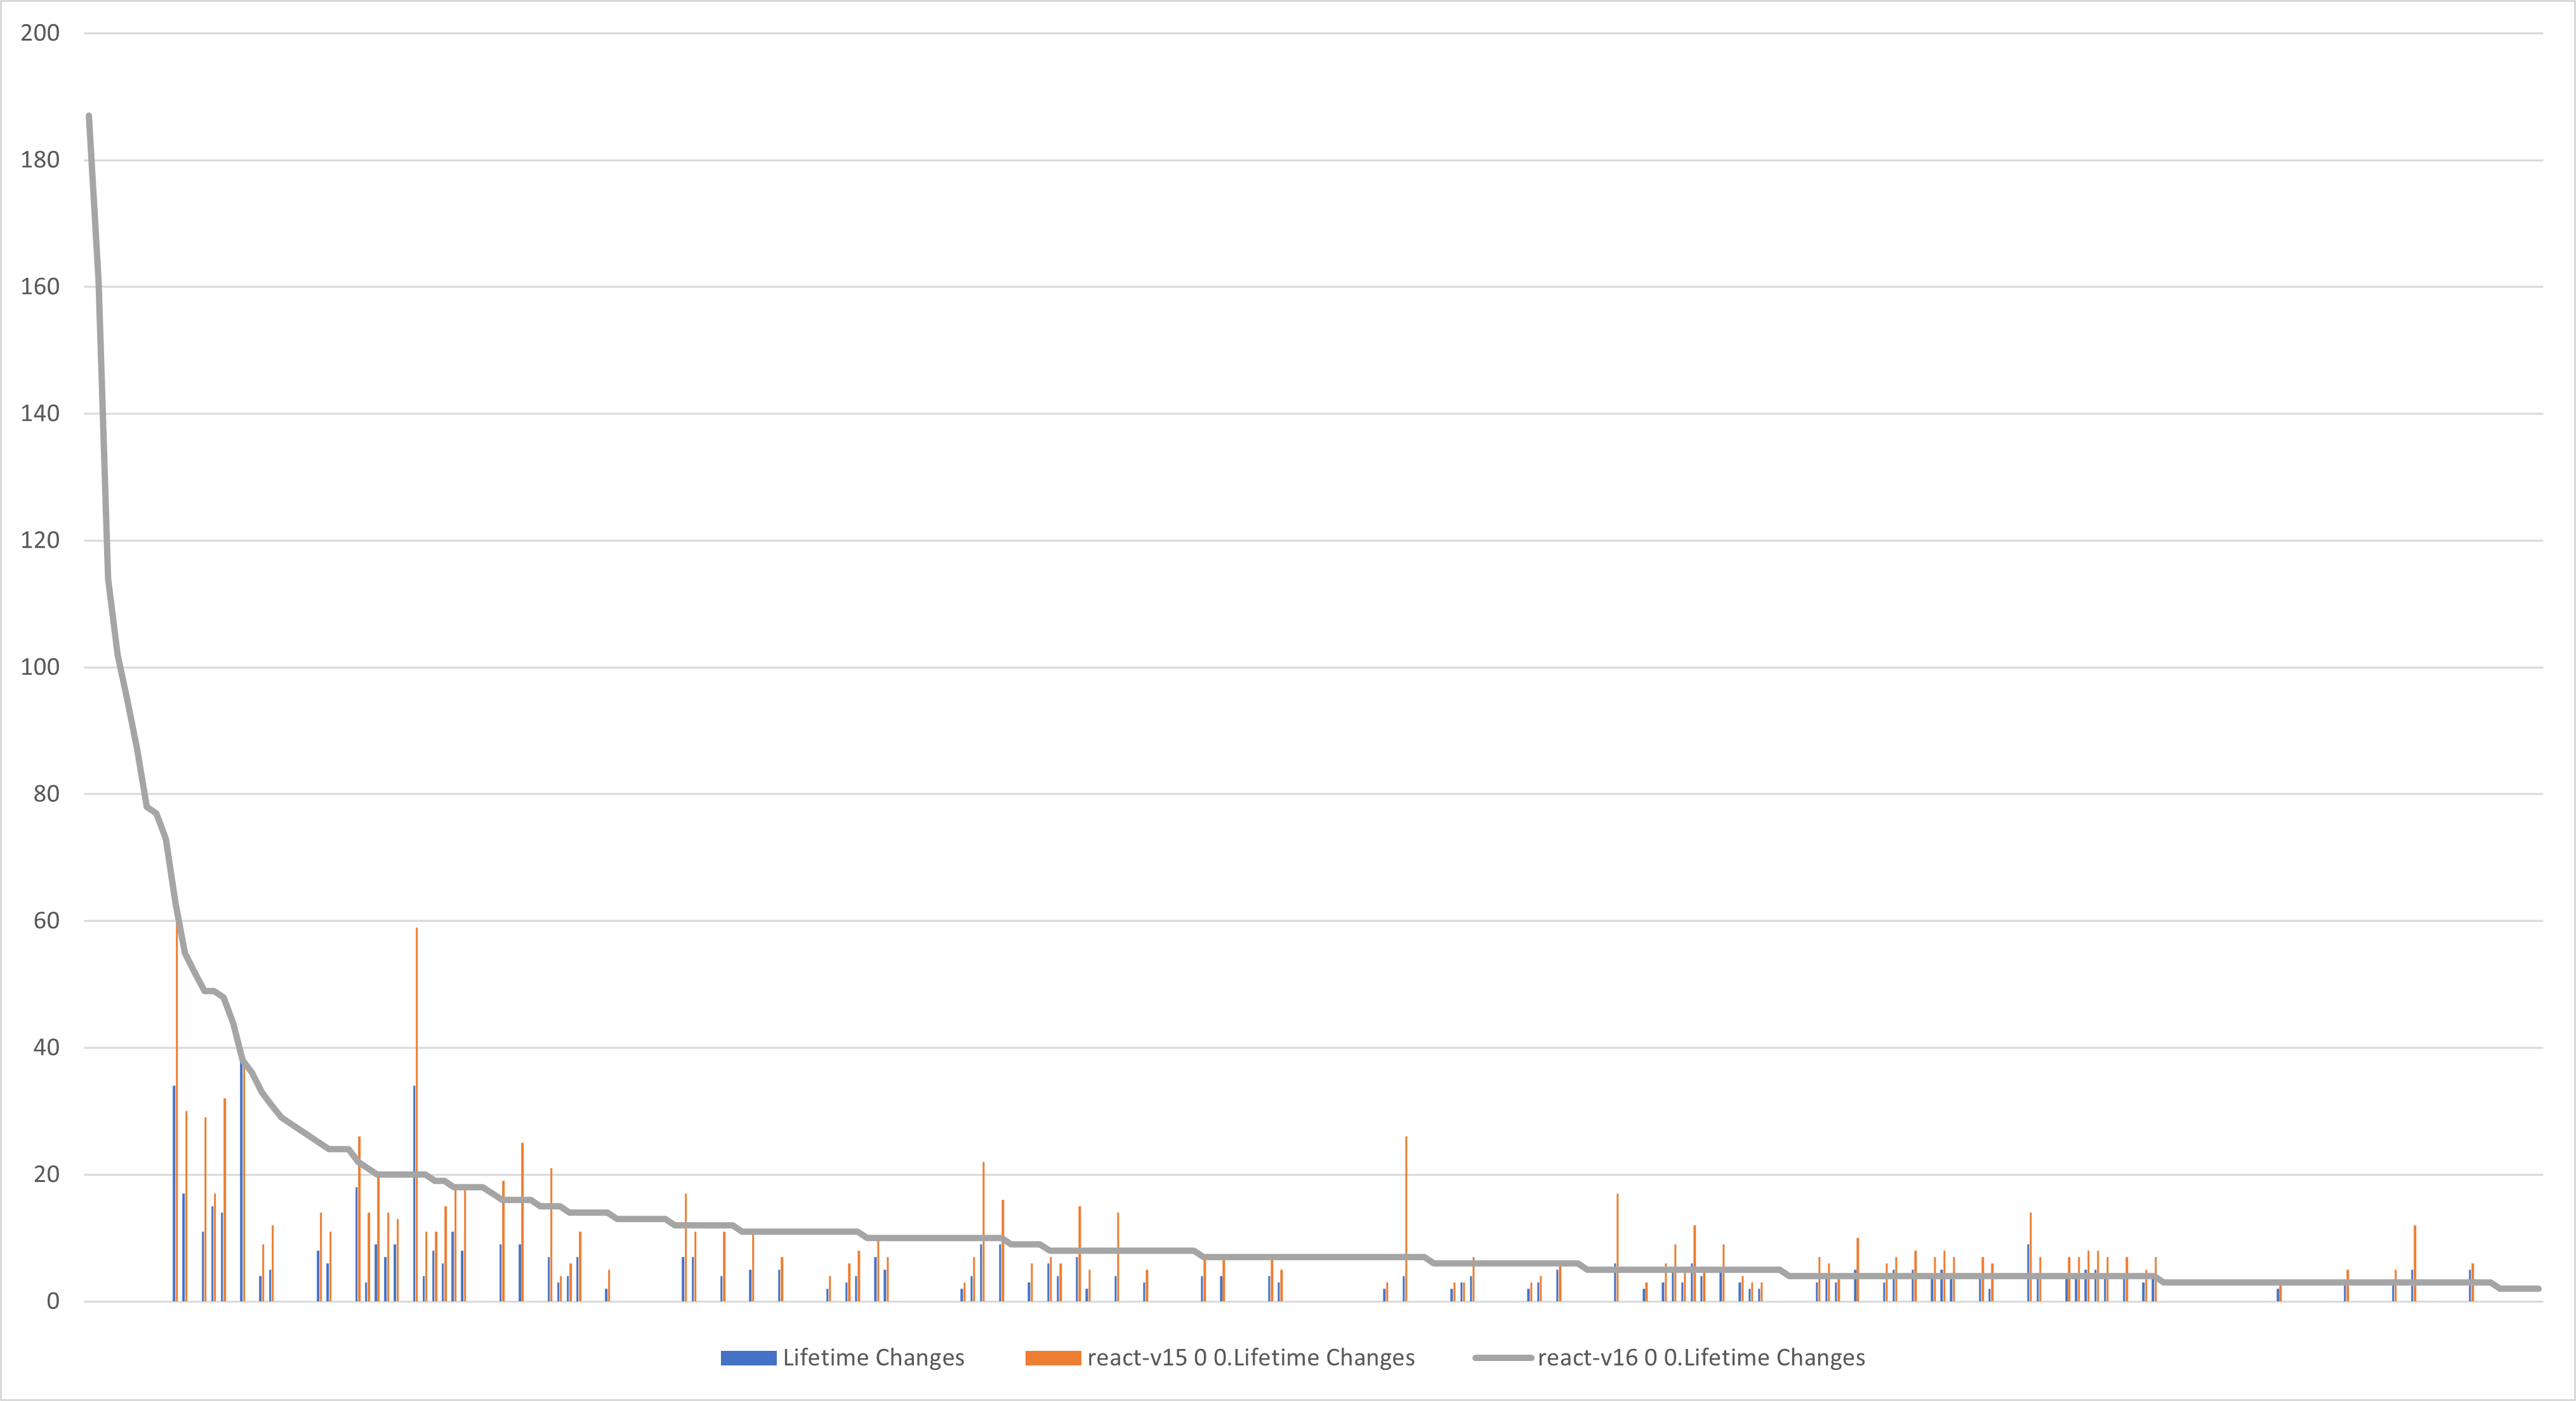
\includegraphics[width=1\textwidth]{images/react/react-all-changes.png}
    \caption{A React teljes kódbázisa a 14-es, 15-ös és 16-os kiadásokban}
    \label{fig:react-all-changes}
\end{figure}